\documentclass[12pt]{article}

\usepackage{sbc-template}

\usepackage{graphicx,url}

%\usepackage[brazil]{babel}   
\usepackage[utf8]{inputenc}  
     
\sloppy

\title{Banco de dados como serviço em tempo real: Firebase}

\author{Fábio da Silva Takaki\inst{1}, Lucas Martins Valladares Ribeiro\inst{1} }


\address{Faculdade de Ciências e Tecnologia\\
  Universidade Estadual Paulista \\
  "Júlio de Mesquita Filho" \\
  Caixa Postal 19060-900  -- Presidente Prudente -- SP -- Brasil
  \email{fabio@takaki.me, lucasmbtos@live.com}
}

\begin{document} 

\maketitle

\begin{abstract}
    Com o surgimento da sociedade digital, diversos conceitos para armazenamento e manipulação dos dados surgiram com a finalidade de diminiuir os custos de recursos e manutenção, do qual destaca-se o Cloud Computing. Este artigo propõe um estudo de caso de uma ferramenta que aborda um dos modelos de serviço da arquitetura Cloud Computing (IaaS, PaaS e SaaS) que é o Firebase, uma ferramenta criada pela Google. O Firebase é uma plataforma mobile que fornece diversos serviços para o rápido desenvolvimento de aplicativos móveis de alta qualidade, do qual destaca-se o serviço de banco de dados em tempo real que será o foco principal deste trabalho.
\end{abstract}
     
\begin{resumo} 
  Este meta-artigo descreve o estilo a ser usado na confeco de artigos e
  resumos de artigos para publicao nos anais das conferncias organizadas
  pela SBC.  solicitada a escrita de resumo e abstract apenas para os artigos
  escritos em portugus. Artigos em ingls devero apresentar apenas abstract.
  Nos dois casos, o autor deve tomar cuidado para que o resumo (e o abstract)
  no ultrapassem 10 linhas cada, sendo que ambos devem estar na primeira
  pgina do artigo.
\end{resumo}


\section{Introdução}

%  descrição do cenário e problemas em aberto
Com a popularização da internet em que surgiu uma sociedade digital, o volume de informações se propagou de forma abundante nos últimos anos. Em decorrência disso, diversos conceitos para armazenamento e manipulação dos dados surgiram com a finalidade de diminuir os custos de recursos e manutenção, no qual destaca-se o Cloud Computing. Cloud computing é uma tecnologia em que os recursos de hardware e software, tais como aplicações especiais, CPU, armazenamento e muitos outros são fornecidos aos usuários através da Internet como um serviço, e é cobrado com base no que você usa \cite{1}. Esses recursos têm a capacidade de escalabilidade automática de acordo com a demanda do cliente.
\\
Este artigo foca em um dos serviços que está em grande crescimento na sociedade moderna que é da área mobile em que mais de 3,2 bilhões de pessoas têm acesso a internet. Firebase é um serviço de dados em nuvem em tempo real, utilizado para criação de aplicativos multiplataformas em que compartilham um banco de dados não relacional que a própria ferramenta disponibiliza. 
\\
Este artigo está organizado da seguinte maneira: na Seção II será apresentado conceitos de Cloud Computing; na Seção III será apresentado a metodologia de desenvolvimento aqui aplicada; na Seção IV um estudo de caso da ferramenta firebase mostrando suas vantagens e desvantagens; por fim na Seção V resultados e trabalhos futuros.

\section{Cloud Computing} \label{sec:firstpage}

O conceito de Cloud Computing é classificado em três modelos de serviço: Software as a Service (SaaS), Plataform as a Service (PaaS) e Infrastructure as a Service (IaaS). Com isso, é possível criar uma pirâmide para representar os modelos de serviço por meio de camadas de virtualização (Figura~\ref{fig:architeture}). Abaixo será descrita brevemente as caracteristicas de cada modelo de serviço para auxiliar o entendimento do que a ferramenta firebase oferece.

\begin{figure}[ht]
\centering
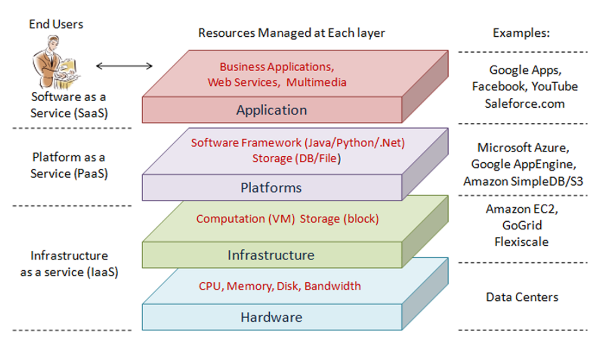
\includegraphics[width=.9\textwidth]{architeture.png}
\caption{Arquitetura Cloud Computing (retirado de: \cite{2})}
\label{fig:architeture}
\end{figure}

\subsection{Infrastructure as a Service}

\subsection{Product as a Service}

\subsection{Software as a Service}
Esse modelo de serviço como o próprio nome diz, é um software como serviço fornecido através da internet, não necessitando de sua instalação. O fornecedor desde modelo de serviço, é responsável por controlar e limitar o uso das aplicações. Portanto, o cliente deste modelo de serviço também fica livre da necessidade de um infraestrutura do qual o fornecedor já disponibiliza.

\section{Metodologia de Desenvolvimento}

In some conferences, the papers are published on CD-ROM while only the
abstract is published in the printed Proceedings. In this case, authors are
invited to prepare two final versions of the paper. One, complete, to be
published on the CD and the other, containing only the first page, with
abstract and ``resumo'' (for papers in Portuguese).

\section{Estudo de Caso}

Section titles must be in boldface, 13pt, flush left. There should be an extra
12 pt of space before each title. Section numbering is optional. The first
paragraph of each section should not be indented, while the first lines of
subsequent paragraphs should be indented by 1.27 cm.

\section{Conclusões e Trabalhos Futuros}

The subsection titles must be in boldface, 12pt, flush left.

\section{Figures and Captions}\label{sec:figs}


Figure and table captions should be centered if less than one line
(Figure~\ref{fig:architeture}), otherwise justified and indented by 0.8cm on
both margins, as shown in Figure~\ref{fig:exampleFig2}. The caption font must
be Helvetica, 10 point, boldface, with 6 points of space before and after each
caption.

\begin{figure}[ht]
\centering
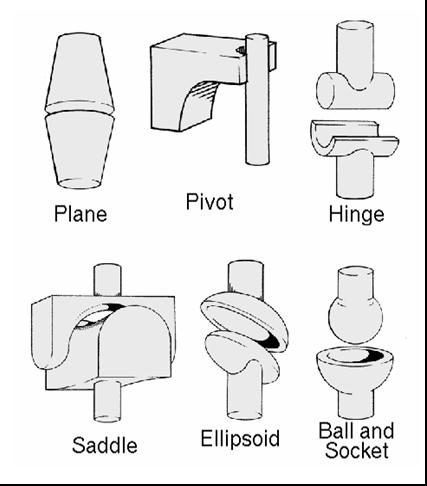
\includegraphics[width=.3\textwidth]{fig2.jpg}
\caption{This figure is an example of a figure caption taking more than one
  line and justified considering margins mentioned in Section~\ref{sec:figs}.}
\label{fig:exampleFig2}
\end{figure}

In tables, try to avoid the use of colored or shaded backgrounds, and avoid
thick, doubled, or unnecessary framing lines. When reporting empirical data,
do not use more decimal digits than warranted by their precision and
reproducibility. Table caption must be placed before the table (see Table 1)
and the font used must also be Helvetica, 10 point, boldface, with 6 points of
space before and after each caption.

\begin{table}[ht]
\centering
\caption{Variables to be considered on the evaluation of interaction
  techniques}
\label{tab:exTable1}
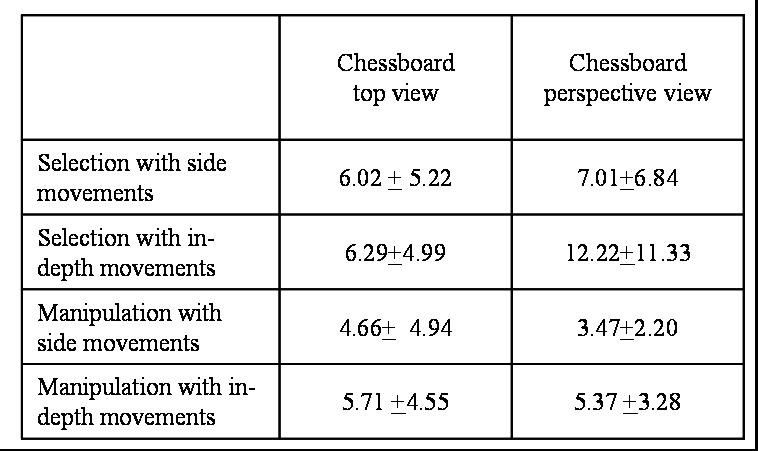
\includegraphics[width=.7\textwidth]{table.jpg}
\end{table}

\section{Images}

All images and illustrations should be in black-and-white, or gray tones,
excepting for the papers that will be electronically available (on CD-ROMs,
internet, etc.). The image resolution on paper should be about 600 dpi for
black-and-white images, and 150-300 dpi for grayscale images.  Do not include
images with excessive resolution, as they may take hours to print, without any
visible difference in the result. 

\section{References}

Bibliographic references must be unambiguous and uniform.  We recommend giving
the author names references in brackets, e.g. Blablabla said Nobody.

The references must be listed using 12 point font size, with 6 points of space
before each reference. The first line of each reference should not be
indented, while the subsequent should be indented by 0.5 cm.

\bibliographystyle{sbc}
\bibliography{bibliografia}

\end{document}
